%!TEX TS-program = xelatex
%!TEX encoding = UTF-8 Unicode
% Awesome CV LaTeX Template for CV/Resume
%
% This template has been downloaded from:
% https://github.com/posquit0/Awesome-CV
%
% Author:
% Claud D. Park <posquit0.bj@gmail.com>
% http://www.posquit0.com
%
% Template license:
% CC BY-SA 4.0 (https://creativecommons.org/licenses/by-sa/4.0/)
%


%-------------------------------------------------------------------------------
% CONFIGURATIONS
%-------------------------------------------------------------------------------
% A4 paper size by default, use 'letterpaper' for US letter
\documentclass[11pt, a4paper]{awesome-cv}

% Configure page margins with geometry
\geometry{left=1.4cm, top=.8cm, right=1.4cm, bottom=1.8cm, footskip=.5cm}

% Specify the location of the included fonts
\fontdir[fonts/]

% Color for highlights
% Awesome Colors: awesome-emerald, awesome-skyblue, awesome-red, awesome-pink, awesome-orange
%                 awesome-nephritis, awesome-concrete, awesome-darknight
\colorlet{awesome}{awesome-orange}
% Uncomment if you would like to specify your own color
% \definecolor{awesome}{HTML}{CA63A8}

% Colors for text
% Uncomment if you would like to specify your own color
% \definecolor{darktext}{HTML}{414141}
% \definecolor{text}{HTML}{333333}
% \definecolor{graytext}{HTML}{5D5D5D}
% \definecolor{lighttext}{HTML}{999999}

% Set false if you don't want to highlight section with awesome color
\setbool{acvSectionColorHighlight}{true}

% If you would like to change the social information separator from a pipe (|) to something else
\renewcommand{\acvHeaderSocialSep}{\quad\textbar\quad}


%-------------------------------------------------------------------------------
%	PERSONAL INFORMATION
%	Comment any of the lines below if they are not required
%-------------------------------------------------------------------------------
% Available options: circle|rectangle,edge/noedge,left/right
% \photo{./examples/profile.png}
\name{}{장회문}
\position{Software Engineer}

\email{palindrom615@hanmail.net}
\github{palindrom615}
\linkedin{palindrom615}

% \gitlab{gitlab-id}
% \stackoverflow{SO-id}{SO-name}
% \twitter{@twit}
% \skype{skype-id}
% \reddit{reddit-id}
% \medium{madium-id}
% \googlescholar{googlescholar-id}{name-to-display}
%% \firstname and \lastname will be used
% \googlescholar{googlescholar-id}{}
% \extrainfo{extra informations}

%-------------------------------------------------------------------------------
\begin{document}

% Print the header with above personal informations
% Give optional argument to change alignment(C: center, L: left, R: right)
\makecvheader[L]

% Print the footer with 3 arguments(<left>, <center>, <right>)
% Leave any of these blank if they are not needed
\makecvfooter
  {\today}
  {장회문~~~·~~~portfolio}
  {\thepage}

%-------------------------------------------------------------------------------
%	CV/RESUME CONTENT
%	Each section is imported separately, open each file in turn to modify content
%-------------------------------------------------------------------------------
%-------------------------------------------------------------------------------
%	SECTION TITLE
%-------------------------------------------------------------------------------
\cvsection{Skills}


%-------------------------------------------------------------------------------
%	CONTENT
%-------------------------------------------------------------------------------
\begin{cvskills}

%---------------------------------------------------------
  \cvskill
    {DevOps} % Category
    {Docker, Docker Swarm, DroneCI} % Skills
    
%---------------------------------------------------------
  \cvskill
    {Infra} % Category
    {Linux, Redis, Nginx, PostgreSQL ...} % Skills

%---------------------------------------------------------
  \cvskill
    {Back-end} % Category
    {Hapi, Typeorm, Tornado, REST API} % Skills

%---------------------------------------------------------
  \cvskill
    {Front-end} % Category
    {ESNext, React, Vue, Redux, Webpack ...} % Skills

%---------------------------------------------------------
  \cvskill
    {Programming} % Category
    {Javascript, Typescript, Python ...} % Skills

%---------------------------------------------------------
  \cvskill
    {Languages} % Category
    {Korean, English, Japanese} % Skills

%---------------------------------------------------------
  \cvskill
    {Tools} % Category
    {Git, Gitlab, Postman, Vim, VScode, Intellij IDEA ...} % Skills

%---------------------------------------------------------
\end{cvskills}

%-------------------------------------------------------------------------------
%	SECTION TITLE
%-------------------------------------------------------------------------------
\cvsection{Honors \& Awards}


%-------------------------------------------------------------------------------
%	SUBSECTION TITLE
%-------------------------------------------------------------------------------


%-------------------------------------------------------------------------------
%	CONTENT
%-------------------------------------------------------------------------------
\begin{cvhonors}

%---------------------------------------------------------
  \cvhonor
    {2차 예선} % Award
    {삼성 대학생 프로그래밍 경진대회(SCPC)} % Event
    {} % Location
    {2018} % Date(s)

%---------------------------------------------------------
\end{cvhonors}

%-------------------------------------------------------------------------------
%	SECTION TITLE
%-------------------------------------------------------------------------------
\cvsection{Projects}


%-------------------------------------------------------------------------------
%	CONTENT
%-------------------------------------------------------------------------------
\begin{cvprojects}

%---------------------------------------------------------
  \cvproject
    {사이버위협관리체계} % title
  	{Feb. 2018 - Feb. 2019} % date
  	{2명} % size
  	{
  	  전군의 인트라넷 및 인터넷 망에 연결되어 있는 PC의 에이전트로부터 사이버 위협 이상징후를 보고받아 수집, 관리자에게 제공하는 프로그램입니다. 원래 python tornado 기반 SSR로 짜여져 있던 것을 nodejs + Typescript와 SPA 기반으로 다시 짰습니다. 약 서100k 정도의 네이티브 윈도우 애플리케이션과의 커넥션이 지속적으로 이어져야 하기 때문에 하위호환을 유지하면서 api를 재설계하는 것이 관건이었습니다.
  	} % description
  	{
  		\begin{cvitems}
  		  \item{팀 내 유일한 풀스택 개발자로서 기획을 확인하면서 시API에 under/over fetching이 없도록 API를 설계했습니다. }
  		  \item{프로젝트를 시작했을 당시 유일한 프론트엔드 개발자로 react 프로젝트의 구조를 잡기 위해 다양한 베스트 프랙티스를 공부했습니다.}
   		  \item{팀에 디자이너가 없어 어쩔 수 없이 외부 컴포넌트 라이브러리를 갖다 썼습니다. SemanticUI를 사용했는데, 그 결정을 하기 위해서 여러 디자인 프레임워크를 비교해보면서 개발자 경험이 어떤지를 파악하려고 노력했습니다.}
   		  \item{사용하고 있는 컴포넌트 라이브러리는 다양한 기능이 별로 없는데 반해 이 프로젝트에서는 트리 구조 등 고수준 UI가 많이 쓰여 상당부분을 react로 직접 구현했습니다.}
  		  \item{성능을 높이기 위해 자주 사용되는 로직에서 redis를 적극 활용했으며 정합성을 유지하기 위해 휘발성 데이터를 분리한다거나, 워커 큐를 도입해 비동기적으로 db에 백업하거나 영속성 설정을 켜는 등 다양한 시도를 해보았습니다. 또 병목을 확인하기 위해 다소 러프하게나마 퍼포먼스를 측정했습니다.}
  		  \item{문서화를 위해 postman을 도입하고, 테스트와 개발 편의성을 위해 ci 서버를 적극 이용했습니다.}
  		  \item{윈도우 애플리케이션과의 호환을 위해 테스트 환경을 구축하고 C\# 코드를 읽었습니다.}
   		  \item{SPA와 WAS 모두 Nginx를 통해 배포하기 위해서 로드밸런싱을 포함해 다양한 Nginx 기능을 활용했습니다.}
   		  \item{폐쇄망에서의 부정기적인 배포, 여러 대의 서버에 배포 등의 상황을 극복하기 위해 docker의 내장기능과 shell 스크립트를 적극 활용했습니다.}
   		  \item{db 암호화 등의 내장 기능을 적극 활용해야 했고, db 마이그레이션을 위해 alembic 등의 솔루션을 고려했으며(결국 raw sql로 썼습니다) 다수의 마이그레이션 코드를 직접 작성했습니다.}
  		\end{cvitems}
  	} % position
  	{} %screenshot
 
%---------------------------------------------------------
  \cvproject
    {Web-Ponies \href{https://github.com/palindrom615/Web-Ponies}{\faGithubSquare}} % title
  	{Oct. 2017 - Feb. 2019} % date
  	{1명} % size
  	{
  	  군에 입대하면서 javascript를 본격적으로 쓰기 시작했을때, 패키지와 모던 문법 등에 익숙해지기 위해 시작한 토이 프로젝트입니다. typescript가 사용됐으며, 브라우저 상에서 pony들이 이리저리 움직이도록 되어 있습니다. 드래그, 터치 등의 이벤트도 구현되어 있습니다.
  	} % description
  	{
  		\begin{cvitems}
  		  \item{2년 가까이 만지다 보면서 저의 실력도 향상해 끊임없이 리팩토링하고 있습니다. 처음에는 브라우저 전역 변수를 통해 상태를 관리하다 객체지향적으로 리팩토링을 하면서 클래스 기반으로 바뀌었습니다. 전역 객체였을 당시의 습관 때문에 하위 클래스에서 상위 클래스를 참조하는 코드가 많았습니다. 이를 해결하기 위해 우선 최상위 싱글턴 클래스를 구현한 뒤 각 클래스들을 이 클래스에 조합해, 의존성 주입을 하는 방식으로 임시적으로 해결했습니다. 책임 연쇄나 퍼사드 등의 디자인 패턴을 활용해 좀더 클래스 간의 의존성을 줄일 수 있을 것 같습니다.}
  		  \item{포니의 이미지와 메타데이터는 github의 다른 리포지터리에서 받아오는데, git submodule을 사용하고, 메타데이터 작성은 nodejs 스크립트를 짜서 사용하고 있습니다.}
  		  \item{리소스의 로딩은 비동기이기는 하지만 병렬은 아닙니다. 나중에 시간이 나면 Promise.all()를 이용해 병렬로 처리하도록 바꾸려고 합니다.}
   		  \item{Typescript의 최신 기능을 활용하려고 노력하며, 덕타이핑은 쓰지 않고 있습니다.}
  		\end{cvitems}
  	} % position
  	{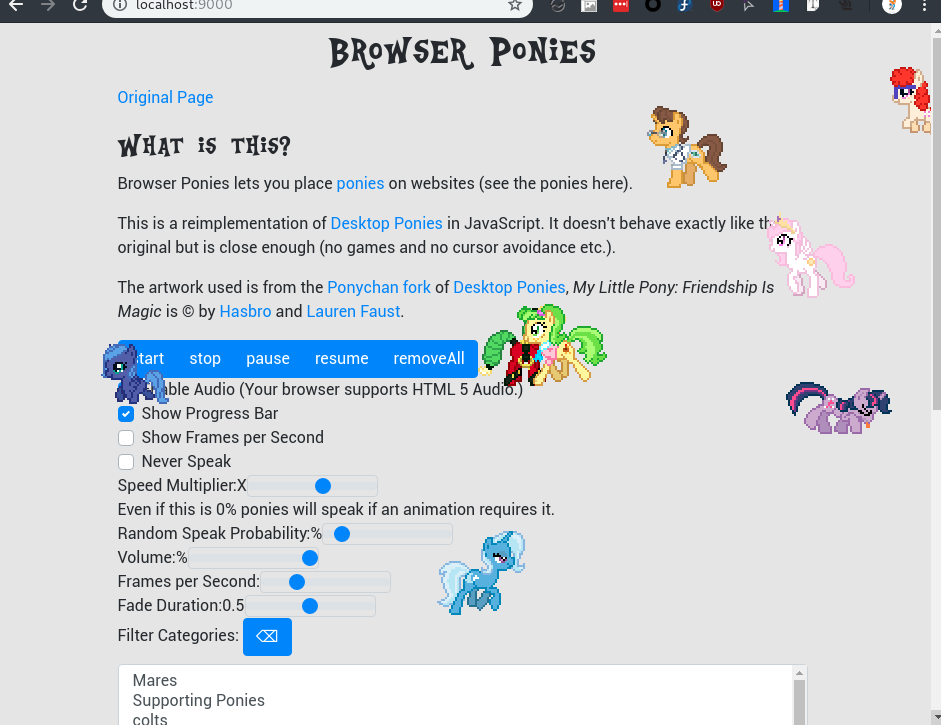
\includegraphics[width=\textwidth]{./cv/webponies}} %screenshot
  	
  	\clearpage
%---------------------------------------------------------
  \cvproject
     {미디어 프레젠테이션 수업 \href{https://github.com/palindrom615/flash-clock-app-demo}{\faGithubSquare}시계 앱
    \href{https://github.com/palindrom615/flash-clock-app-demo}{\faGithubSquare}하루버퍼} % title
  	{Sep. 2016 - Dec. 2016} % date
  	{1명} % size
  	{
  	  현재 저는 대학에서 공업디자인 부전공을 하고 있습니다. 위 두 앱은 디자인 수업 수강 당시 과제로 제출한 것입니다.
  	} % description
  	{
  		\begin{cvitems}
  		  \item{간단한 모바일 앱 프로토타입 작성이 목표인 수업이었습니다. 빠른 프로토타입을 만들고 UX를 중점적으로 체크하는 수업이었습니다. 툴은 어도비 플래시와 Actionscript를 사용했습니다. 애니메이션 관련 라이브러리로는 둘 모두 greensock을 사용했습니다.}
  		  \item{첫 번째 앱은 중간 과제로 만든 시계 앱입니다. 한 프레임만큼 시간이 흐를 때마다 시간을 갱신합니다. 또 화면을 감싸는 빨간 줄과 그 끝의 빨간 점은 현재 하루의 얼마만큼 시간이 갔는지 표시해줍니다. 저걸 계산하는 것이 상당히 어려웠는데, 일단 동그란 시계과 같은 각도를 가리키도록 표시하면 전체 하루 길이에 비해 6시/18시 경에는 하루가 빨리 가는 것처럼 느껴지는데 반해 오전 4시나 10시 정도에는 느리게 가는 것처럼 느껴지는데 이 왜곡의 정도가 심합니다. 그래서 각도가 아니라 길이를 사용해도록 해야 했는데, 되도록 하드코딩을 지양하면서 다양한 디바이스에서 너비/높이를 런타임에서 확인하고 또 직선과 점이 직사각형을 두르는 방식으로 가도록 하는 것이 가장 난이도 있는 작업이었습니다.}
  		  \item{시계 앱에서 화면 가운데 있는 버튼을 누르면 전체 색깔이 마치 css transition처럼 자연스럽게 바뀌도록 되어 있습니다.}
  		  \item{다음은 기말 과제로 만든 하루버퍼라는 앱입니다. 본인의 기분을 선택하고, 140자 이내로 글자를 써서 제출하면 로그를 남기는 일종의 일기장같은 기믹을 가진 앱입니다.}
  		  \item{화면 위쪽의 긴 직사각형을 누르면 로그와 글쓰기 화면이 전환되는데, 자연스러운 애니메이션을 위해서 별도로 액티비티를 만드는 게 아니라 서로 이어붙여서 디스플레이의 위치만 이동하는, 말하자면 magic scroll같은 형태로 되어 있습니다.}
  		  \item{140자라는 constraint를 유지하기 위해서 제출할 때 한 번, 로그를 쌓을 때 한 번 확인합니다. 자연스러운 UX를 위해 140자를 넘겼을 때 어떤 식으로든 제한됨을 표시해야 하는데, 트위터처럼 글자 수를 빨갛게 표시하고 제출 버튼을 disable한 정도로 처리했습니다.}
  		\end{cvitems}
  	} % position
  	{} %screenshot
  	\vskip 0.2in
    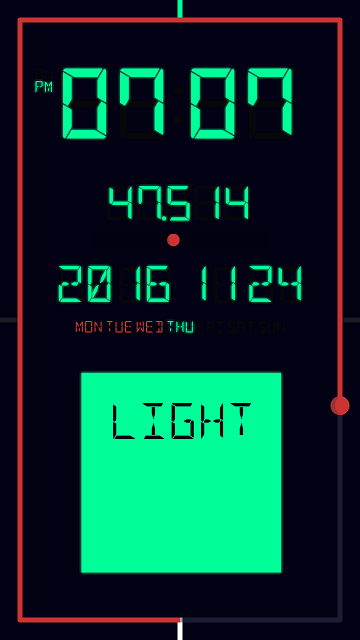
\includegraphics[width=0.3\textwidth]{./cv/clock}
    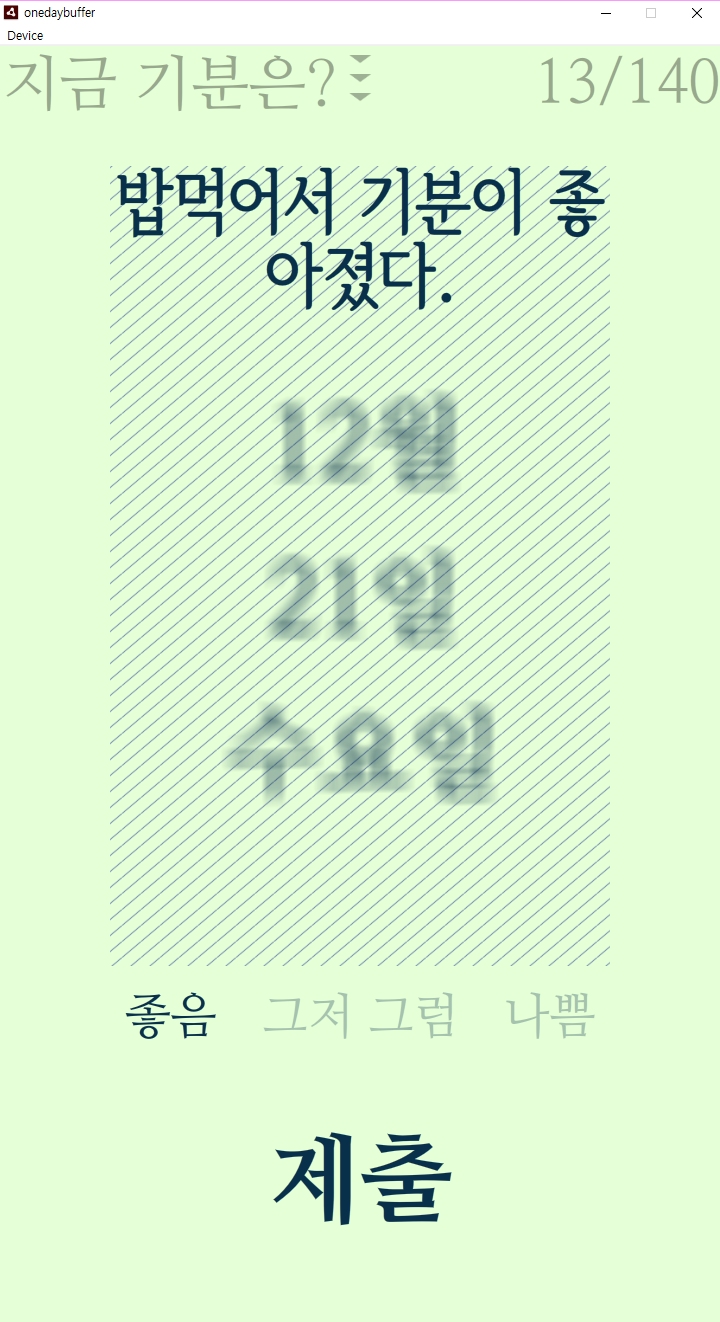
\includegraphics[width=0.3\textwidth]{./cv/onedaybuff1}
    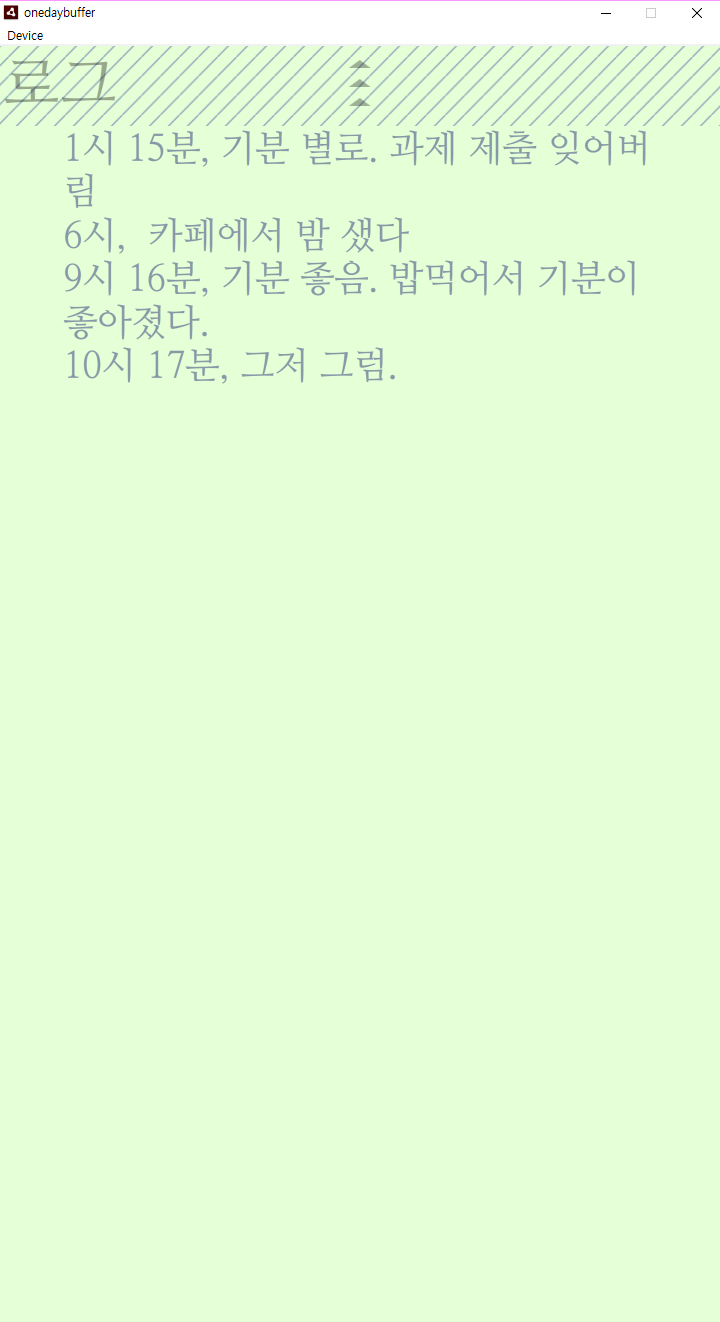
\includegraphics[width=0.3\linewidth]{./cv/onedaybuff2}
\clearpage
%---------------------------------------------------------
  \cvproject
    {카카오페이 경력기술서, 포트폴리오 \href{https://github.com/palindrom615/Awesome-CV}{\faGithubSquare}} % title
  	{Jan. 2019} % date
  	{1명} % size
  	{
  	  짧은 시간 안에 빠르게 만들 수 있고, 일정한 퀄리티를 보장받으며, 프로그래머블한 방식으로 경력기술서 및 포트폴리오를 작성할 방법을 찾다가 깃허브에서 훌륭한 \TeX 템플릿이 있는 것을 발견하고 빠르게 작성해 보았습니다.
  	} % description
  	{
  		\begin{cvitems}
  		  \item{\TeX{}는 처음 써봤는데, 오래된 소프트웨어라서 그런지 패키지 관리가 굉장히 어렵다는 인상을 받았습니다. 또, html처럼 컨텐츠와 스타일을 분리시키려 하지 않아서 코드가 뒤섞여있다는 인상을 받았습니다.}
  		  \item{css보다 자유롭게 스타일을 바꾸기 위해서 스타일을 마크업과 합치는 대신 \TeX{}에서는 전역변수와 매크로를 적극적으로 활용해서 보일러플레이트를 줄이고 문서의 구조화를 시키는데, 매크로때문에 자칫 코드의 가독성이 망칠 수도 있다는 생각이 듭니다. }
  		  \item{원래 Curriculum Vitae를 작성하기 위해서 만든 템플릿이라서 프로젝트 중심의 구조가 없어 테이블 기반의 cvproject 매크로를 직접 간단히 만들어 보았습니다. 몇가지 상수도 수정했습니다. }
  		  \item{매크로끼리 체이닝도 되고, 매크로 여러 개를 중첩하는 구조가 lisp를 연상시켰습니다. 동적 언어라서 자꾸 컴파일 오류가 나는데, 함수 정의가 문법적으로 너무 어려운 것 같습니다.}
  		  \item{나중에 시간이 나면 포트폴리오를 정리하면서 만든 양식을 정리해 원본 리포지터리에 PR를 낼 계획입니다.}
  		\end{cvitems}
  	} % position
  	{} %screenshot
    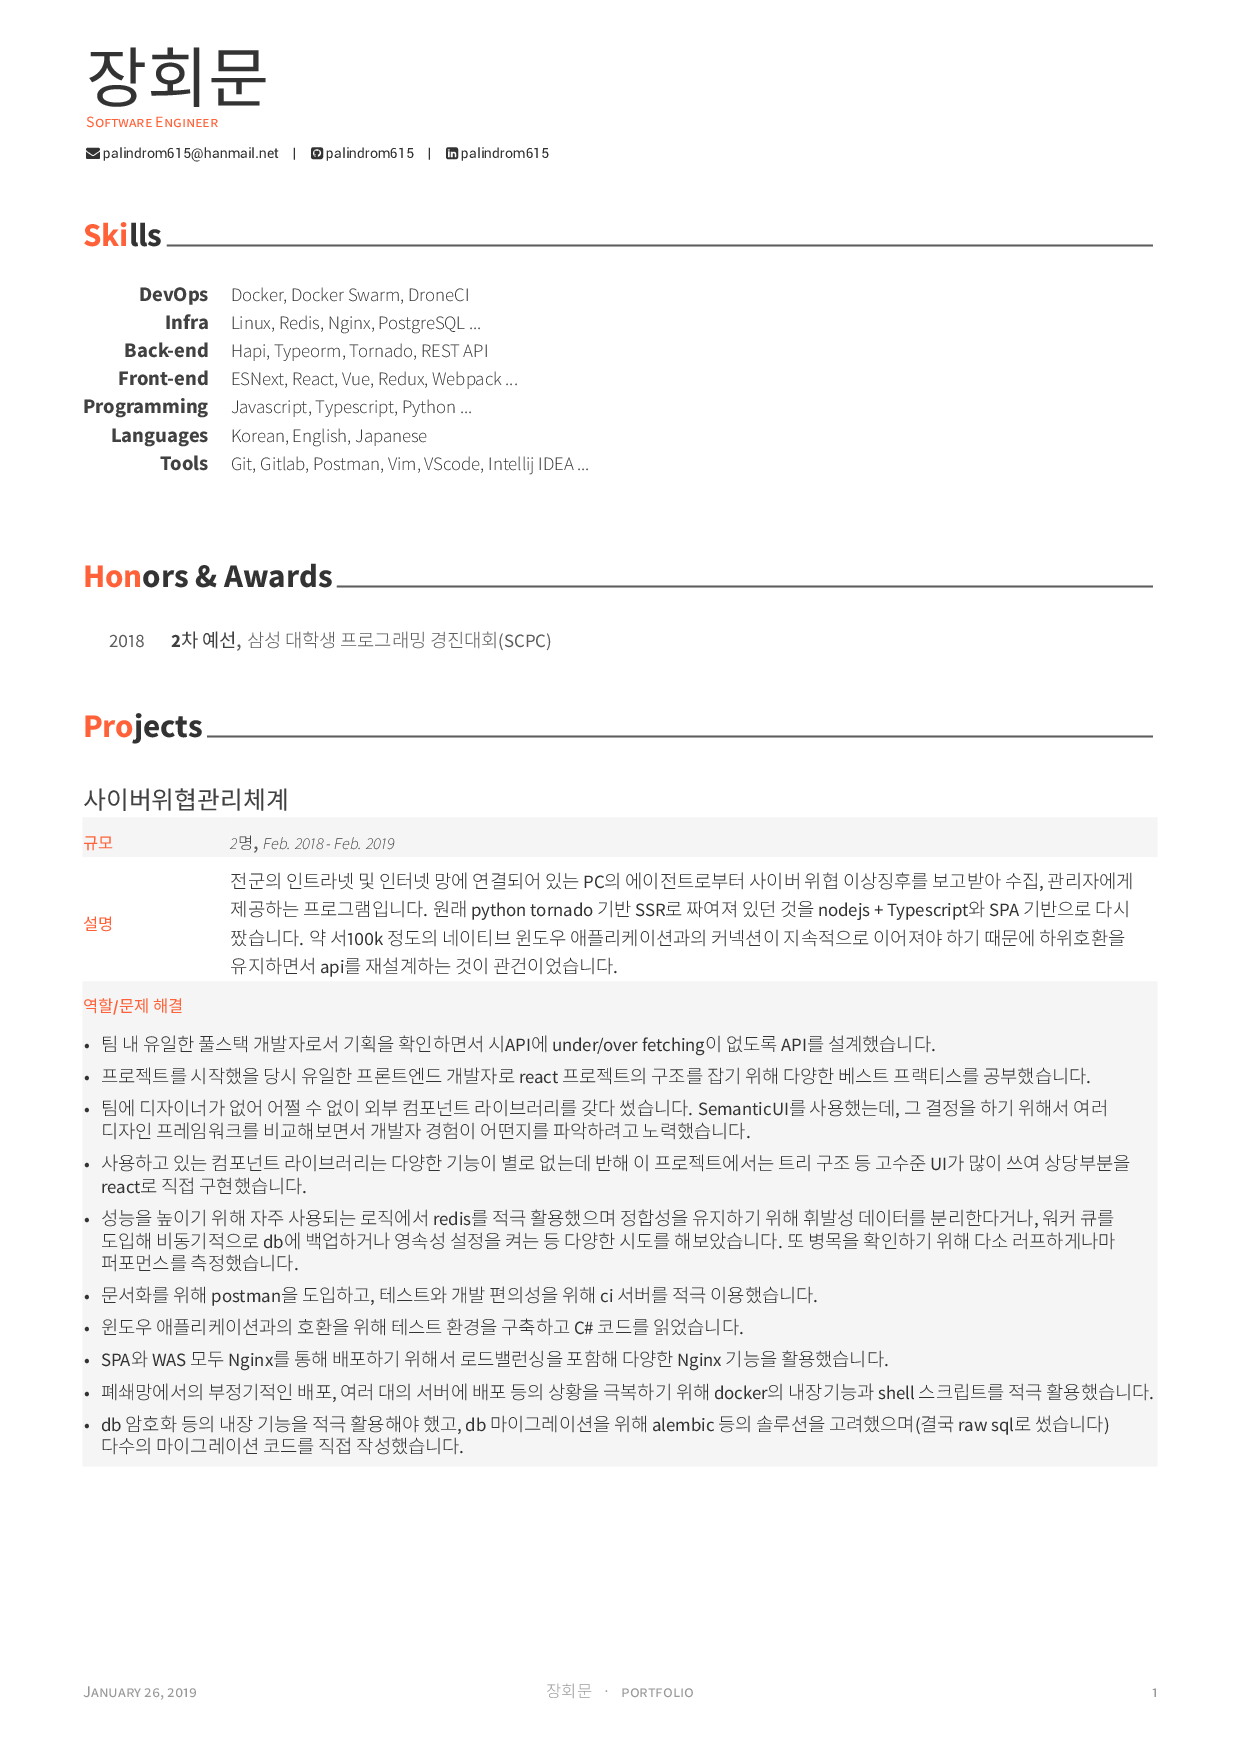
\includegraphics[width=0.4\textwidth]{./cv/cv1}
    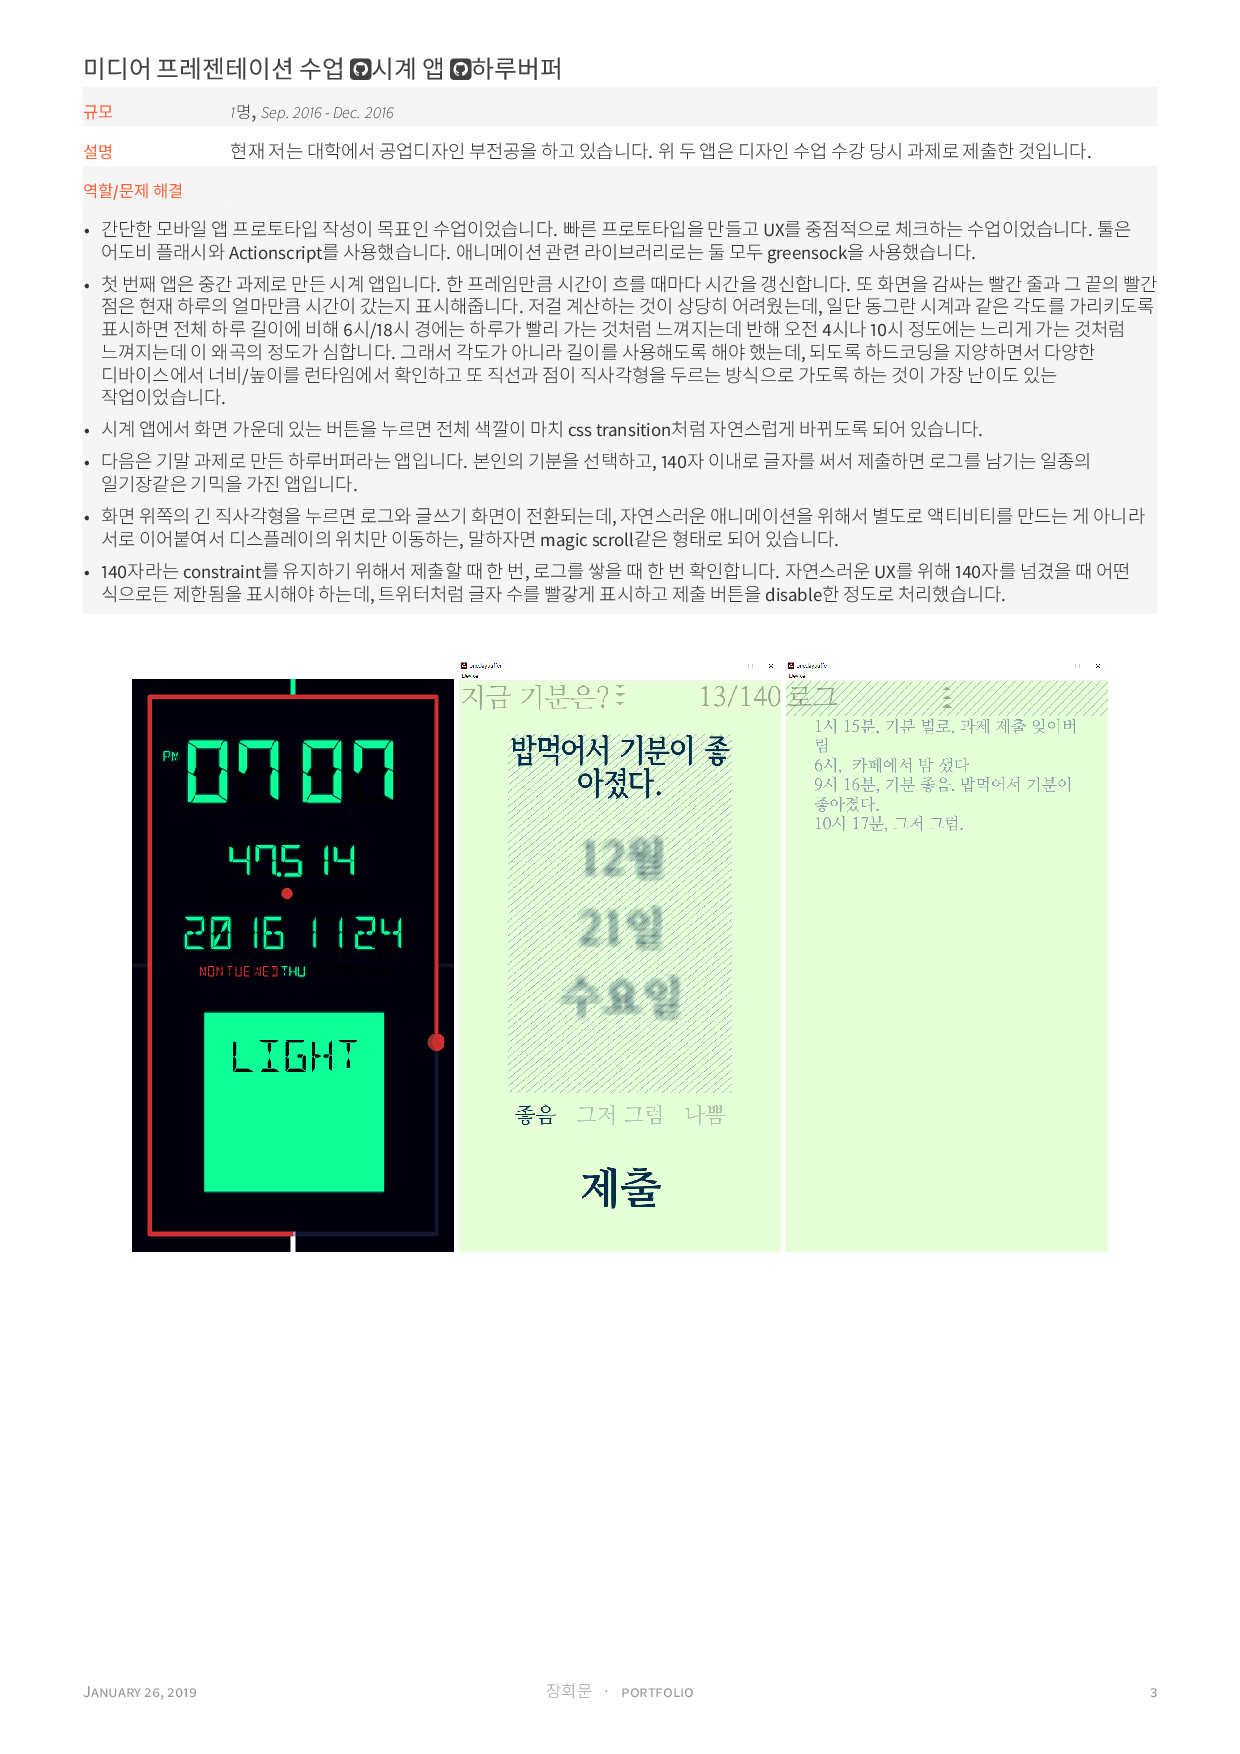
\includegraphics[width=0.4\textwidth]{./cv/cv2}  	  	
  	  	
\end{cvprojects}


%-------------------------------------------------------------------------------
\end{document}
